\documentclass[twoside,a4paper]{book}

\usepackage[dvipdfm]{graphicx}
\usepackage[dvipdfm]{hyperref}
\usepackage[utf8]{inputenc}
\usepackage{authblk}
\usepackage{float}
\usepackage{longtable}
\usepackage{minted}

\author[1]{Mart Lubbers}
\author[2]{Francisco Torreira}
\affil[1]{\url{mart.lubbers@mpi.nl}}
\affil[2]{\url{francisco.torreira@mpi.nl}}
\title{Praatalign: an interactive Praat plug-in for performing phonetic forced
alignment\\\large A detailed manual}
\date{\today} 
\hypersetup{
	pdftitle={Praatalign detailed manual},
	pdfauthor={Mart Lubbers and Francisco Torreira},
	pdfsubject={Praatalign},
	pdfproducer={Mart Lubbers},
	pdfkeywords={praat,htk,phonetic forced alignment},
	hidelinks
}

\newcommand{\tabitem}{~~\llap{\textbullet}~~}
\definecolor{bg}{rgb}{0.95,0.95,0.95}
\newminted{latex}{
	bgcolor=bg,
	fontfamily=tt,
	fontsize=\footnotesize,
	tabsize=2
}

\begin{document}
\maketitle
\cleardoublepage
\setcounter{page}{1}
\tableofcontents
\chapter{Introduction}
\section{Introduction}
Praatalign is a plug-in for Praat that can be used to do forced phonetic
alignment on speech signals and in particular free speech. Praatalign combines
the powerful HTK toolkit

\section{Example workflow}
\begin{figure}[H]
	\centering
	\includegraphics[width=\linewidth]{./img/s1.eps}
	\caption{Opening and selecting a \texttt{LongSound} and a \texttt{TextGrid}}
\end{figure}

\begin{figure}[H]
	\centering
	\includegraphics[width=\linewidth]{./img/s2.eps}
	\caption{Press \texttt{View \& Edit}}
\end{figure}

\begin{figure}[H]
	\centering
	\includegraphics[width=\linewidth]{./img/s2a.eps}
	\caption{Press \texttt{Setup force alignment...}}
\end{figure}

\begin{figure}[H]
	\centering
	\includegraphics[width=\linewidth]{./img/s3.eps}
	\caption{Edit the settings to your liking}
\end{figure}

\begin{figure}[H]
	\centering
	\includegraphics[width=\linewidth]{./img/s4.eps}
	\caption{Because of the dictionary flag a dialog spawns}
\end{figure}

\begin{figure}[H]
	\centering
	\includegraphics[width=\linewidth]{./img/s5.eps}
	\caption{Select the dictionary}
\end{figure}

\begin{figure}[H]
	\centering
	\includegraphics[width=\linewidth]{./img/s6.eps}
	\caption{Select an interval, zoom in and press
	\texttt{Align the current interval}}
\end{figure}

\begin{figure}[H]
	\centering
	\includegraphics[width=\linewidth]{./img/s7.eps}
	\caption{Wait a couple of seconds and see the alignment. Note that I have
enabled the spectrogram during the alignment. This makes the aligner
significantly faster. Note that there is an error because of a reduction from
\texttt{cuidado} to \texttt{cuida}.}
\end{figure}

\begin{figure}[H]
	\centering
	\includegraphics[width=\linewidth]{./img/s8.eps}
	\caption{After changing the annotation error with the reduction to
\texttt{cuida(do)} because the Spanish phonetizer knows of a truncation
construction via braced syllables. The we run the alignment again the results
are much better. If this is a common truncation we could add a
pronunciation variant of if it is really general we could create a ruleset
file}
\end{figure}

\chapter{Installation}
\section{Preparation}
Some programs are not included in the package due to licencing and
compatibility restrictions and need to be pre-installed in order for the
plug-in to work properly. The following list of programs need to be installed.
\begin{itemize}
	\item \textbf{Praat}\\
		Praat is a program that allows you to do phonetic analysis and annotations
		with a computer and praatalign uses Praat to provide an interactive user
		interface to the annotated sound files. Praat can be downloaded
		here\footnote{\url{http://www.fon.hum.uva.nl/praat}}.
	\item \textbf{Python}\\
		Python is used to interpret the scripts that run the core of the aligner.
		Python, in this case Python 2, can be downloaded
		here\footnote{\url{https://www.python.org/download/}}. Be sure to download
		the Python 2 version as the Python 3 version is not supported.
	\item \textbf{SoX}\\
		For processing the sound files in a very detailed and controlled way we
		use SoX. Although Praat also has sound processing capabilities SoX works
		better, this is because Praat does not allow you to specify certain options
		like sampling rate for all formats. Sox can be downloaded
		here\footnote{\url{http://sox.sourceforge.net/}}.
	\item \textbf{Hcopy \& HVite}\\
		HCopy and HVite are programs from the HTK toolkit and due to licencing
		issues we can not provide the binaries in a direct way. The program is for
		free but you are not allowed to distribute it. For Windows there is a
		compiled binary package, for Linux and Mac you have to compile the package
		yourself. For windows we tested the version that is available after
		registering here\footnote{\url{
http://htk.eng.cam.ac.uk/ftp/software/htk-3.3-windows-binary.zip}}.
		For Linux and Mac the latest compiled sources that work can be found
		here\footnote{\url{http://htk.eng.cam.ac.uk/ftp/software/HTK-3.4.tar.gz}}.
		Installing HTK is probably the hardest part of using the program, if it
		does not work you can always contact us.
\end{itemize}

\section{Installation}
\label{sec:installation}
The installation of the plug-in is very easy but for all operating systems a bit
different. For every main operating system there is an installation script that
automates the installation.
\paragraph{Automated installation}\strut\\
Run the installation script:
\begin{itemize}
	\item \textbf{Linux}\\
		\texttt{./install\_lin}
	\item \textbf{Mac}\\
		\texttt{./install\_mac}
	\item \textbf{Windows}\\
		\texttt{install\_win.bat}
\end{itemize}

\paragraph{Manual installation}\strut\\
Copy the contents of the root directory to:
\begin{itemize}
	\item \textbf{Linux}\\
		\texttt{\$\{HOME\}/.praat-dir/plugin\_pralign}.
	\item \textbf{Windows}\\
		\texttt{\%USERPROFILE\%\textbackslash Praat\textbackslash plugin\_pralign}
	\item \textbf{Mac}\\
		\texttt{\$\{HOME\}/Library/Preferences/Praat Prefs/plugin\_pralign}.
\end{itemize}

\chapter{Documentation}
\section{General information}
Presets for Spanish, Tzeltal, English and Dutch are included. Presets for
Australian English, Estonian, German, Hungarian, Italian, New Zealand English
Polish and Portuguese will be added in the future. When you want a language
from the above list implemented with priority you can always contact us. If you
want other languages you can still contact us and it might be possible using
the SAMPA model.

Dictionary, ruleset and all other files are, and should be, encoded in
\texttt{UTF-8}. To enforce this the plug-in changes the default behaviour of
Praat every time Praat loads to make sure Praats reading and
writing preferences are set to \texttt{UTF-8}.
When the plug-in is successfully installed several menu items are added in the
\texttt{TextGrid} editor under the \texttt{Interval} menu. The options for
alignment only work when you are editing a \texttt{TextGrid} and a
\texttt{LongSound}. It does not work with a normal \texttt{Sound}, this is
because \texttt{Sound} objects are loaded in memory and thus detached from the
real sound file on disk. Currently it is also only tested on \texttt{WAVE}
files.

\section{Menu items}
\begin{itemize}
	\item \texttt{Generate dictionary from tier}\\
		This functions allows the user to generate a dictionary containing all the
		missing or unphonetizable words within a file. The program will prompt for
		a file location where the dictionary file will be stored. Only the missing
		words from the current selected tier are written to the file. When this
		process is done the user can fill the dictionary with pronunciations.

		For this function to work \texttt{Setup forced alignment...} has to run
		at least once.
	\item \texttt{Clean selection}\\
		This function is a helper function to clean up old or wrong alignment. When
		the function runs all annotation data within the selection within the
		selected tier will be removed. Note that this is not necessary to do before
		an alignment because this function runs by default before the alignment of
		an interval.
	\item \texttt{Align current interval}\\
		This function aligns the current selected interval on the current selected
		tier. When selecting a small interval it should not take much time at all.
		Be careful that you do not try to align an output tier from a previous
		alignment(word or phone level). When this happens you will be prompted to
		make sure you mean to align an output tier.

		For this function to work \texttt{Setup forced alignment...} has to run
		at least once.
	\item \texttt{Align current tier}\\
		This function aligns the entire selected tier. Note that this can take
		quite a long time for long data. When you do not have a lot of
		pronunciation variants it still can take about $30$ minutes for an hour
		long conversation. This function will clear the tier entirely before
		aligning.

		For this function to work \texttt{Setup forced alignment...} has to run
		at least once.
	\item \texttt{Setup forced alignment...}\\
		When you run this function a big option menu is spawned that will generate
		the necessary settings files that are needed for the alignment. For almost
		all functions this functions has to run at least once before they can run.
		When you close the form a settings file is written to disk.

		All options start with a long description and then a letter code
		describing the internal variable, the following options identified by their
		letter code can be specified in the settings menu:
		\begin{itemize}
			\item \texttt{new}\\
				Name of the tier where the phone level alignment is stored, this can be
				either an existing tier or a non existing tier. If the tier does not
				exist it will be created upon doing the first alignment. If the tier
				does exist the annotations that overlap with the alignment will be
				removed.
			\item \texttt{wrd}\\
				Name of the tier that stores the word level alignment, this can be
				again either an existing tier or a non existing tier with the same
				consequences as for the \texttt{new} value. In theory this tier can be
				the same tier as the \texttt{new} tier, however this can and will
				result in unexpected behaviour and will generate a warning every time
				you align something.
			\item \texttt{lan}\\
				Language used for the force alignment, all properly added languages
				will appear in this drop down list. Currently only Spanish, Tzeltal,
				Dutch and English are supported.
			\item \texttt{dic}\\
				Flag for setting a dictionary file, when you tick this box you
				will be prompted to locate the dictionary file. When a dictionary was
				previously set an extra variable is shown named \texttt{dictionary}
				containing the path to the current dictionary. When you want to change
				the dictionary you can either tick the \texttt{dic} box or change the
				path in the \texttt{dictionary} field. To unset a dictionary you can
				just clear out the \texttt{dictionary} field and leave the \texttt{dic}
				box unticked.
			\item \texttt{rul}\\
				Flag for setting a ruleset file, when you tick this box you will be
				prompted to locate the ruleset file. When a ruleset file was
				previously set an extra variable is shown named \texttt{ruleset}
				containing the path to the current ruleset file. When you want to
				change the ruleset file you can either tick the \texttt{rul} box or
				change the path in the \texttt{ruleset} field. To unset a ruleset file
				you can just clear out the \texttt{ruleset} field and leave the
				\texttt{rul} box unticked.
			\item \texttt{thr}\\
				Extra margin used for every annotation, when the annotations are placed
				to close to the real sound the initial pause can clobber up the
				beginning of speech and that can reduce the aligners performance.
				Setting the \texttt{thr} value to $0.1$ will for example increase all
				boundaries from annotations with $100$ms. Note that this does not
				change the original annotation and it will only increase the widen the
				annotation when there is room to do so, meaning that it will not create
				overlap with other annotations.
			\item \texttt{log}\\
				Location of the log output, when an annotation is aligned a log is
				produced that contains detailed output of all the subcommands and can
				be used for debugging purposes. You can either put a file path in here
				that will become the log file or if you want to discard the log you can
				put \texttt{/dev/null} there on Linux or Mac and \texttt{nul} on
				Windows.
			\item \texttt{sox}\\
				Flag for setting a custom SoX executable location, when you tick this
				box you will be prompted to locate a SoX executable. When a SoX
				executable is already present in one of the location in \texttt{\$PATH}
				on Linux or mac or \texttt{\%PATH\%} on Windows you do not have to set
				a custom location. When a custom location has been previously set an
				extra variable named \texttt{soxex} is shown that contains the current
				custom SoX location.  When you want to change this you can either tick
				the \texttt{sox} box or change the path in the \texttt{soxex} field.
				When you want to unset a custom SoX location you can just clear out the
				\texttt{soxex} field and leave the \texttt{sox} box unticked.
			\item \texttt{hvite}\\
				Flag for setting a custom HVite executable location, when you tick this
				box you will be prompted to locate a HVite executable. When a HVite
				executable is already present in one of the location in \texttt{\$PATH}
				on Linux or mac or \texttt{\%PATH\%} on Windows you do not have to set
				a custom location. When a custom location has been previously set an
				extra variable named \texttt{hviteex} is shown that contains the
				current custom HVite location.  When you want to change this you can
				either tick the \texttt{sox} box or change the path in the
				\texttt{hviteex} field.  When you want to unset a custom HVite location
				you can just clear out the \texttt{hviteex} field and leave the
				\texttt{hvite} box unticked.
			\item \texttt{hcopy}\\
				Flag for setting a custom HCopy executable location, when you tick this
				box you will be prompted to locate a HCopy executable. When a HCopy
				executable is already present in one of the location in \texttt{\$PATH}
				on Linux or mac or \texttt{\%PATH\%} on Windows you do not have to set
				a custom location. When a custom location has been previously set an
				extra variable named \texttt{hcopyex} is shown that contains the
				current custom HCopy location.  When you want to change this you can
				either tick the \texttt{sox} box or change the path in the
				\texttt{hcopyex} field.  When you want to unset a custom HCopy location
				you can just clear out the \texttt{hcopyex} field and leave the
				\texttt{hcopy} box unticked.
		\end{itemize}
\end{itemize}

\section{Dictionary}
To phonetize words praatalign either uses the provided phonetizer or a
dictionary. Dictionaries are plain text files that contain words and one or
more pronunciations. A dictionary file is a \texttt{UTF-8} encoded file
containing non-empty lines separated by a newline
character\footnote{\label{fn:n1}On Linux and Mac this is default, on Windows
this can cause problems. When using praatalign on windows please refrain to a
text editor that has newline capabilities like Notepad++}. Lines starting with
a \texttt{\#} will be ignored and can thus be used as comments. The format of a
dictionary entry is a word followed by a tab followed by tab separated
pronunciations. An example dictionary can be found in
Listing~\ref{lst:example_dictionary}

\begin{listing}
	\caption{Example dictionary}
	\label{lst:example_dictionary}
	\begin{minted}[tabsize=4]{text}
# This is comment
# This is a word with two possible pronunciations
ado	a d o	a o
# These are words with one possible pronunciation
empatar	e m p a t a r
empataran	e m p a t a r a n
	\end{minted}
\end{listing}
	
\section{Ruleset}
Besides generating pronunciation by using the dictionary and phonetization you
can also use rulesets to define pronunciation variants. Ruleset make you able
to define general rules applied over all words(phonetized words and dictionary
words). In this way you can easily define for example deletion rules.
Internally the pronunciation variants are visualized as a graph. With rulesets
you can define shortcuts within that graph. For example the word \texttt{ado}
and rule: \texttt{(?P<fr>a)d(?P<to>o)} make the graph in
Figure~\ref{fig:ruleset_example}. A Ruleset file is a \texttt{UTF-8} encoded
file containing non-empty lines separated by a newline character. Lines
starting with a \texttt{\#} will be ignored and can thus be used as comments.
The format of a ruleset entry is just the regular expression describing the
rule. The regular expression uses two named groups to tie certain character
groups to each other. The group \texttt{fr} marks the start node and the group
\texttt{to} marks the destination node.  Several escape sequences besides the
standard escape sequences exist, namely:
\begin{itemize}
	\item \texttt{\textbackslash v} for vowels(\texttt{[aoeiu]})
	\item \texttt{\textbackslash c} for consonants(\texttt{[\textasciicircum aoeiu]})
	\item \texttt{\#} for a inter word silence
\end{itemize}

\begin{figure}[H]
	\label{fig:ruleset_example}
	\centering
	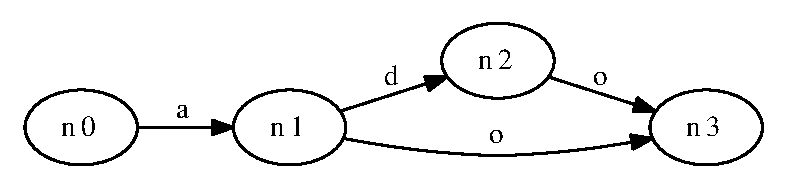
\includegraphics[scale=0.3]{./fig_ruleset_example.eps}
	\caption{Example result of \texttt{ado->ao} deletion}
\end{figure}

\section{Supported languages information}
Different languages have different possibilities within the possibilities of
phonetizing and dictionaries. Some languages are impossible to phonetize and
thus need a complete dictionaries. Some languages can be fully phonetized and
only need a dictionary for foreign words.

\subsection{Dutch}
A detailed description of the Dutch phones can be found in
Section~\ref{sec:sldutch}. Further specification:
\begin{table}[H]
	\caption{Dutch language properties}
	\begin{tabular}{ll}
		Phonetizer support & None\\
		Ruleset support & Full\\
		Dictionary support &  Full
	\end{tabular}
\end{table}

\subsection{English}
A detailed description of the English phones can be found in
Section~\ref{sec:slenglish}
\begin{table}[H]
	\caption{Dutch language properties}
	\begin{tabular}{ll}
		Phonetizer support & None\\
		Ruleset support & Full\\
		Dictionary support &  Full
	\end{tabular}
\end{table}
There is conversion script for the English CMU
dictionary\footnote{\url{http://www.speech.cs.cmu.edu/cgi-bin/cmudict}} located
in \texttt{./par.eng/cmu2praatalign.py} that converts the CMU dictionary to
praatalign format. The scripts is a Python script and should download the
dictionary if you haven't done it yourself and will write it to a
\texttt{dict.eng} file by default. The usage is: \texttt{python
cmu2praatalign.py [inputfile [outputfile]]}.

\subsection{Tzeltal}
Tzeltal uses the general SAMPA models and information about the phones can be
your in Section~\ref{sec:slsampa}. Further specification:
\begin{table}[H]
	\caption{Tzeltal language properties}
	\begin{tabular}{ll}
		Phonetizer support & Full\\
		Ruleset support & Full\\
		Dictionary support &  Full
	\end{tabular}
\end{table}

\subsection{Spanish}
A detailed description of the Spanish phones can be found in
Section~\ref{sec:slspanish}. Further specification:
\begin{table}[H]
	\caption{Spanish language properties}
	\begin{tabular}{ll}
		Phonetizer support & Full\\
		Ruleset support & Full\\
		Dictionary support &  Full
	\end{tabular}
\end{table}
\section{Scriptability and Batch processing}
Although the praatalign script is inherently interactive it is still possible
to batch process corpora using simple praat scripts. To facilitate this
function a file called \texttt{\$DIR/settings\_ni.praat} can be run where
\texttt{\$DIR} is the location of the plugin files. The location of the plugin
files for your operating system can be found in Section~\ref{sec:installation}
in the manual installation text. The \texttt{settings\_ni.praat} is a stripped
down version of the settings dialog present in the aligner. Since it is using a
praat form to ask for the user input, in contrary to the pause dialog in the
normal settings scirpt, it can be run non interactively by running the script
from a praat script.

For example if you want to setup the aligner to align a tzeltal file with all
custom values on linux under the user frobnicator you can put this in your
script to setup the aligner:

\begin{flushleft}
	\texttt{
runScript: "/home/frobnicator/.praat-dir/plugin\_pralign/settings\_ni.praat",\\
..."custom\_phone\_tier", "custom\_word\_tier", "/some/path/to/dict",\\
..."/some/path/to/ruleset", 0, "tze", "no", "/some/path/to/logfile",\\
..."/usr/bin/sox", "/usr/bin/HVite", "/usr/bin/HCopy"}
\end{flushleft}

When you then open a \texttt{TextGrid} and a \texttt{LongSound} file and do
\texttt{View \& Edit} to open the editor you can run the alignment from the
script using the button text as function. For example the script could look
like the script in Listing~\ref{lis:scriptab}.

\begin{listing}
	\caption{Example scriptability}
	\label{lis:scriptab}
	\centering
	\begin{minted}[bgcolor=bg,fontfamily=tt,fontsize=\footnotesize,tabsize=2]{text}
# We assume the LongSound and TextGrid are selected previously

# Spawn the editor
View & Edit

# Open the editor
editor: "TextGrid " + objectname$
	# This bit of code is a small snippet to select a specific tier with the
	# index: tiernum, tiernum is obtained by querying all tiers outside the
	# editor and finding the tier that matches the name
	currenttiernum = -1
	while currenttiernum <> tiernum
		Select next tier
		inf$ = Editor info
		currenttiernum = extractNumber(inf$, "Selected tier: ")
	endwhile
	
	# Generate the settings file
	runScript: "/home/frobnicator/.praat-dir/plugin_pralign/settings_ni.praat",
..."custom_phone_tier", "custom_word_tier", "/some/path/to/dict",
..."/some/path/to/ruleset", 0, "tze", "no", "/some/path/to/logfile",
..."/usr/bin/sox", "/usr/bin/HVite", "/usr/bin/HCopy"
	
	# Do the actual alignment
	Align current tier
	# When this is done aligned data can be found in: custom_phone_tier and 
	# custom_word_tier. $
endeditor
	\end{minted}
\end{listing}

\chapter{Extending praatalign}
\section{Introduction}
Extending the aligner with new languages should be very easy for languages that
can be mapped on the current SAMPA model or on any other available model(maus
model).
Adding a language with a new model could be possible but no support will be
given, however you can always try, you can even try getting help. Adding a
language requires a couple of components that need to be written or adapted.

\section{Phonetizer}
Phonetization of your language is the most elegant solution of translating the
graphemes to phonemes. Implementing a phonetizer is as easy as implementing one
function called \texttt{phonetizeword}. A skeleton class can be found in
\texttt{phonetizer.py}. The function in the skeleton class is accompanied by
comments. A phonetized utterance is always of the following form:\\
\texttt{utt=[word1, word2, ..., wordn]}, 
\texttt{word=[pron1, pron2, ..., pronn]} and
\texttt{pron=[phone1, phone2, ..., phonen]} and every phone is a string.
So if you want to use the skeleton class with the \texttt{phonetizeword}
function you need to return a list of lists of strings where every
string is a phone from the model. If you also want to do utterance based
translation you need to return a list of lists of lists of strings.

\section{Dictionary}
If you do not want to use a phonetizer you can also suffice with only using a
dictionary based translation. Dictionary based translation still needs to be
loaded as a phonetizer though. All phonetizers include also a dictionary based
lookup. In the \texttt{phonetizer.py} a dictionary phonetizer is already
present called \texttt{PhonetizerDictionary}. There is also a loopback
phonetizer that takes the literal annotation as transcription. This phonetizer
is currently not used but could be used when an exact phonetic translation is
already available.

\section{Injecting the aligner}
When you have the translation from grapheme to phoneme the only thing that
needs to be done is adding it to the script files.
\begin{itemize}
	\item \texttt{phonetizer.py}\\
		On the bottom of this file there is a dictionary containing all the
		translations from language code to phonetizer and parameters directory. You
		need to add your language to that dictionary.
	\item \texttt{settings.praat}\\
		In this file you need to add stuff on multiple locations, namely within the
		second \texttt{if} that relies in the first outer \texttt{if} block you
		need to add your language with its appropriate position. When you want your
		language on top you need to adapt the other numbers too.

		Finally within the \texttt{pause} block you need to add your language code
		in the \texttt{optionMenu:} block on the same position as specified
		earlier.
\end{itemize}
When you have changed these files properly your language should be available in
the menus and work out of the box.

\chapter{Appendices}
\section{How to cite}
\begin{listing}[H]
	\centering
	\caption{Bibtex snippet}
	\begin{latexcode}
@misc{praatalign,
	author={Lubbers, Mart and Torreira, Francisco},
	title={Praatalign: an interactive Praat plug-in for performing phonetic forced alignment},
	howpublished={\url{https://github.com/dopefishh/praatalign}},
	year={2013-2014},
	note={Version 1.0}
}
	\end{latexcode}
\end{listing}

\newpage
\section{Dutch phone specification}
\label{sec:sldutch}
Mapping with SAMPA
alphabet\footnote{\url{http://www.phon.ucl.ac.uk/home/sampa/dutch.htm}}

\paragraph{Consonants}
\subparagraph{Plosives}\strut\\
\begin{tabular}{llll}
	Praatalign & SAMPA & Word & Praatalign Transcription\\
	\hline
		p & p & pak & p A k\\
		b & b & bak & b A k\\
		t & t & tak & t A k\\
		d & d & dak & d A k\\
		k & k & kap & k A p\\
		g & g & goal & g o: l
\end{tabular}

\subparagraph{Fricatives}\strut\\
\begin{tabular}{llll}
	Praatalign & SAMPA & Word & Praatalign Transcription\\
	\hline
	f & f & fel & f E l\\
	v & v & vel & v E l\\
	s & s & sein & s E i n\\
	z & z & zijn & z E i n\\
	x & x & toch & t o x\\
	G & G & goed & G u t\\
	h & h & hand & h A n t\\
	Z & Z & bagage & b A g a: Z @\\
	S & S & show & S o: u
\end{tabular}

\subparagraph{Sonorants}\strut\\
\begin{tabular}{llll}
	Praatalign & SAMPA & Word & Praatalign Transcription\\
	\hline
	m & m & met & m E t\\
	n & n & net & n E t\\
	N & N & bang & b A N\\
	l & l & land & l A n t\\
	r & r & rand & r A n t\\
	w & w & wit & w I t\\
	j & j & ja & j a:
\end{tabular}

\paragraph{Vowels}
\subparagraph{Checked}\strut\\
\begin{tabular}{llll}
	Praatalign & SAMPA & Word & Praatalign Transcription\\
	\hline
	I & I & pit & p I t\\
	E & E & pet & p E t\\
	A & A & pat & p A t\\
	O & O & pot & p O t\\
	Y & Y & put & p Y t\\
	@ & @ & gemakkelijk & G @ m A k @ l @ k
\end{tabular}

\subparagraph{Free}\strut\\
\begin{tabular}{llll}
	Praatalign & SAMPA & Word & Praatalign Transcription\\
	\hline
	i & i & vier & v i r\\
	y & y & vuur & v y r\\
	u & u & voer & v u r\\
	a: & a: & naam & n a: m\\
	e: & e: & veer & v e: r\\
	P2: & 2: & deur & d P2: r\\
	o: & o: & voor & v o: r\\
	EI & Ei & fijn & f EI n\\
	P9y & 9y & huis & h P9y s\\
	Au & Au & goud & x Au t
\end{tabular}

\subparagraph{Diphthongs}\strut\\
\begin{tabular}{llll}
	Praatalign & SAMPA & Word & Praatalign Transcription\\
	\hline
	a:i & a:i & draai & d r a: i\\
	o:i & o:i & mooi & m o: i\\
	ui & ui & roeiboot & r ui b o: t\\
	iu & iu & nieuw & n iu\\
	yu & yu & duw & d yu\\
	e:u & e:u & sneeuw & s n e: u
\end{tabular}

\subparagraph{Marginals}\strut\\
\begin{tabular}{llll}
	Praatalign & SAMPA & Word & Praatalign Transcription\\
	\hline
	E: & E: & cr\'eme & k r E: m\\
	P9: & 9: & freule & f r P9: l @\\
	O: & O: & roze & r O: z @
\end{tabular}

\newpage
\section{English phone specification}
\label{sec:slenglish}
\begin{longtable}{llp{0.4\textwidth}ll}
	Praatalign & SAMPA & Phonetics & Examples & ISO639-3\\
	\hline
	\textless usb\textgreater &  & human noise, garbage &  & xxx\\
	\textless nib\textgreater &  & noise, non-human &  & xxx\\
	\textless p:\textgreater &  & silence interval &  & xxx\\
	a~ & a~ & nasalized central open vowel & vent & fra\\
	E~ & E~ & nasalized lengthened front half open unrounded vowel &  & deu\\
	o~ & o~ & nasalized back half closed rounded vowel & bon & fra\\
	3: & 3: & lengthened front half open unrounded vowel & furs & eng\\
	i: & i: & lengthened front closed unrounded vowel &  mieten & deu\\
	6: & 6: & lengthened central neutral unrounded vowel &  & aus\\
	\}: & \}: & lengthened central closed rounded vowel & pool & aus\\
	e: & e: & lengthened front half closed unrounded vowel & mehr & deu\\
	o: & o: & lengthened back half closed rounded vowel & Sohle & deu\\
	u: & u: & lengthened back closed rounded vowel & Hut & deu\\
	A: & A: & lengthened back open unrounded vowel & stars & eng\\
	O: & O: & lengthened back half open rounded vowel & cause & eng\\
	@\} & @\} & diphthong &  & eng\\
	Ae & Ae & diphthong &  & aus\\
	\{I & \{I & diphthong &  & aus\\
	\{O & \{O & diphthong &  & aus\\
	oI & oI & diphthong &  & aus\\
	eI & eI & diphthong & raise & eng\\
	aI & aI & diphthong & Bein & deu\\
	OI & OI & diphthong & noise & eng\\
	@U & @U & diphthong & nose & eng\\
	aU & aU & diphthong & Haus & deu\\
	I@ & I@ & diphthong & dears & eng\\
	e@ & e@ & diphthong & stairs & eng\\
	U@ & U@ & diphthong & cures & eng\\
	tS & tS & voiceless postalveolar affricate & English chair & xxx\\
	dZ & dZ & voiced postalveolar affricate & English gin & xxx\\
	e & e & front half closed unrounded vowel & US English bear & xxx\\
	\{ & \{ & front open unrounded vowel & English cat & xxx\\
	Q & Q & back open rounded vowel & British English not, cough & xxx\\
	O & O & back half open rounded vowel & British English law & xxx\\
	V & V & back half open unrounded vowel & RP and US English run & xxx\\
	U & U & back closed rounded vowel somewhat more centralised and relaxed & English put, Buddhist & xxx\\
	@ & @ & central neutral unrounded vowel & English about, winner & xxx\\
	i & i & front closed unrounded vowel & English see & xxx\\
	u & u & back closed rounded vowel & English soon & xxx\\
	o & o & back half closed rounded vowel & US English sore & xxx\\
	E & E & front half open unrounded vowel & English bed & xxx\\
	6 & 6 & central neutral unrounded vowel & German besser & xxx\\
	p & p & voiceless bilabial plosive & English pen & xxx\\
	b & b & voiced bilabial plosive & English but & xxx\\
	t & t & voiceless alveolar plosive & English two & xxx\\
	d & d & voiced alveolar plosive & English do & xxx\\
	k & k & voiceless velar plosive & English skill & xxx\\
	g & g & voiced velar plosive & English go & xxx\\
	f & f & voiceless labiodental fricative & English fool & xxx\\
	v & v & voiced labiodental fricative & English voice & xxx\\
	T & T & voiceless dental fricative & English thing & xxx\\
	D & D & voiced dental fricative & English this & xxx\\
	s & s & voiceless alveolar fricative & English see & xxx\\
	z & z & voiced alveolar fricative & English zoo & xxx\\
	S & S & voiceless postalveolar fricative & English she & xxx\\
	Z & Z & voiced postalveolar fricative & English pleasure & xxx\\
	h & h & voiceless glottal fricative & English ham & xxx\\
	m & m & bilabial nasal & English man & xxx\\
	n & n & alveolar nasal & English no & xxx\\
	N & N & velar nasal & English ring & xxx\\
	r & r & alveolar trill & Spanish perro & xxx\\
	l & l & alveolar lateral approximant & English left & xxx\\
	w & w & labial-velar approximant & English we & xxx\\
	j & j & palatal approximant & English yes & xxx\\
	I & I & front closed unrounded vowel, but somewhat more centralised and relaxed, in Polish: mid closed unrounded & English city & xxx\\
	? & ? & glottal stop & German Verein & xxx\\
	x & x & voiceless velar fricative & Scots loch & xxx\\
	C & C & voiceless palatal fricative & German Ich & xxx\\
	W & W & voiceless labial-velar fricative &  & xxx\\
	\textless &  & recording initial silence &  & xxx\\
	\textgreater &  & recording trailing silence &  & xxx\\
	\# &  & inter-word silence &  & xxx\\
\end{longtable}

\newpage
\section{SAMPA phone specification}
\label{sec:slsampa}
\begin{longtable}{lllll}
%\caption{SAMPA phone specification table}
	Praatalign & SAMPA & Phonetics & Example & ISO6393-9\\
	\hline
	i: & i: & lengthened front closed unrounded vowel & mieten & deu\\
	ii & ii & lengthened front closed unrounded vowel & riisu & ekk\\
	e: & e: & lengthened front half closed unrounded vowel & mehr & deu\\
	ee & ee & lengthened front half closed unrounded vowel & keere & ekk\\
	E: & E: & lengthened front half open unrounded vowel & Mär & deu\\
	y: & y: & lengthened front closed rounded vowel & Tür & deu\\
	2: & 2: & lengthened front half closed rounded vowel & Höhle & deu\\
	a: & a: & lengthened central open vowel & Haar & deu\\
	u: & u: & lengthened back closed rounded vowel & Hut & deu\\
	o: & o: & lengthened back half closed rounded vowel & Sohle & deu\\
	3: & 3: & lengthened front half open unrounded vowel & furs & eng\\
	A: & A: & lengthened back open unrounded vowel & stars & eng\\
	O: & O: & lengthened back half open rounded vowel & cause & eng\\
	6: & 6: & lengthened central neutral unrounded vowel & & aus\\
	\}: & \}: & lengthened central closed rounded vowel & pool & aus\\
	9: & 9: & lengthened front half open rounded vowel & & nld\\
	\{\{ & \{\{ & lengthened front open unrounded vowel & kääru & ekk\\
	yy & yy & lengthened front closed rounded vowel & müüri & ekk\\
	22 & 22 & lengthened front half closed rounded vowel & nööri & ekk\\
	uu & uu & lengthened back closed rounded vowel & kuuri & ekk\\
	oo & oo & lengthened back half closed rounded vowel & poori & ekk\\
	77 & 77 & back half closed unrounded vowel & sõõre & ekk\\
	AA & AA & lengthened back open unrounded vowel & vaaru & ekk\\
	aU & aU & diphthong & Haus & deu\\
	aI & aI & diphthong & Bein & deu\\
	ai & ai & diphthong & & ita\\
	a:i & a:i & diphthong & & nld\\
	Ae & Ae & diphthong & & aus\\
	Au & Au & diphthong & & nld\\
	OY & OY & diphthong & heulen & deu\\
	eI & eI & diphthong & raise & eng\\
	e@ & e@ & diphthong & stairs & eng\\
	ei & ei & diphthong & & ita\\
	e:i & e:i & diphthong & & nld\\
	eU & eU & diphthong & & por\\
	EI & EI & diphthong & raise & eng\\
	Ei & Ei & diphthong & & ita\\
	\{I & \{I & diphthong & & aus\\
	\{O & \{O & diphthong & & aus\\
	I@ & I@ & diphthong & dears & eng\\
	Ii: & Ii: & diphthong & accede & aus\\
	i:@ & i:@ & diphthong & memorial & nze\\
	io & io & diphthong & & ita\\
	iu & iu & diphthong & & nld\\
	ja & ja & diphthong & & ita\\
	jo & jo & diphthong & & ita\\
	ju & ju & diphthong & & ita\\
	oI & oI & diphthong & & aus\\
	oi & oi & diphthong & & ita\\
	o:i & o:i & diphthong & & nld\\
	oU & oU & diphthong & & por\\
	oE & oE & diphthong & & ita\\
	OI & OI & diphthong & noise & eng\\
	Oi & Oi & diphthong & & ita\\
	ue & ue & diphthong & & ita\\
	ui & ui & diphthong & & nld\\
	U@ & U@ & diphthong & cures & eng\\
	wa & wa & diphthong & & ita\\
	we & we & diphthong & & ita\\
	wi & wi & diphthong & & ita\\
	wO & wO & diphthong & & ita\\
	yu & yu & diphthong & & nld\\
	@U & @U & diphthong & nose & eng\\
	@\} & @\} & diphthong & & eng\\
	9y & 9y & diphthong & & nld\\
	QI & QI & diphthong & abide & aus\\
	U\} & U\} & diphthong & abuse & aus\\
	VU & VU & diphthong & acetone & aus\\
	Vi & Vi & diphthong & abased & aus\\
	\{o & \{o & diphthong & accounts & aus\\
	2i & 2i & diphthong & & ekk\\
	2i: & 2i: & diphthong & & ekk\\
	7o: & 7o: & diphthong & & ekk\\
	7u: & 7u: & diphthong & & ekk\\
	7u & 7u & diphthong & & ekk\\
	Ai & Ai & diphthong & & ekk\\
	Ai: & Ai: & diphthong & & ekk\\
	Ao: & Ao: & diphthong & & ekk\\
	Au: & Au: & diphthong & & ekk\\
	Ae: & Ae: & diphthong & & ekk\\
	ei: & ei: & diphthong & & ekk\\
	e:u & e:u & diphthong & & nld\\
	i~ & i~ & nasalized front closed unrounded vowel & & xxx\\
	e~ & e~ & nasalized front half closed unrounded vowel & vin & fra\\
	a~ & a~ & nasalized central open vowel & vent & fra\\
	o~ & o~ & nasalized back half closed rounded vowel & bon & fra\\
	9~ & 9~ & nasalized front half open rounded vowel & neuv & fra\\
	E~ & E~ & nasalized lengthened front half open unrounded vowel & & deu\\
	O~ & O~ & nasalized back half open rounded vowel & & deu\\
	u~ & u~ & nasalized back closed rounded vowel & & xxx\\
	a:~ & a:~ & nasalized lengthened central open vowel & & deu\\
	E:~ & E:~ & nasalized lengthened front half open unrounded vowel & & deu\\
	o:~ & o:~ & nasalized lengthened back half closed rounded vowel & & deu\\
	O:~ & O~ & nasalized lengthened back half open rounded vowel & & nld\\
	ts\_j & ts' & palatalized voiceless alveolar affricate & c'ma & pol\\
	dz\_j & dz' & palatalized voiced alveolar affricate & dz'wig & pol\\
	s\_j & s' & palatalized voiceless alveolar fricative & syk & pol\\
	z\_j & z' & palatalized voiced alveolar fricative & zbir & pol\\
	n\_j & n' & palatalized alveolar nasal & kon' & pol\\
	l\_j & l' & palatalized alveolar lateral approximant & pali & ekk\\
	t\_j & t' & palatalized voiceless alveolar plosive & padi & ekk\\
	d\_j & d' & voiced alveolar plosive English & gyár & hun\\
	g\_j & g' & palatalized voiced velar plosive & Gienek & pol\\
	x\_j & x' & palatalized voiceless velar fricative & hiacynt & pol\\
	k\_j & k' & palatalized voiceless velar plosive & kierowca & pol\\
	p\_j & p' & palatalized voiceless bilabial plosive & piasek & pol\\
	tt\_j & t't & palatalized long voiceless alveolar plosive & pati & ekk\\
	ss\_j & s's & palatalized long voiceless alveolar fricative & kassi & ekk\\
	nn\_j & n'n & palatalized long alveolar nasal & panni & ekk\\
	ll\_j & l'l & palatalized alveolar lateral approximant & palli & ekk\\
	p\_h & p\_h & aspirated voiceless bilabial plosive & & spa\\
	t\_h & t\_h & aspirated voiceless alveolar plosive & & spa\\
	k\_h & k\_h & aspirated voiceless velar plosive & & spa\\
	tt & tt & geminate of t & fatto & ita\\
	pp & pp & geminate of p & & ita\\
	kk & kk & geminate of k & & ita\\
	dd & dd & geminate of d & & ita\\
	gg & gg & geminate of g & & ita\\
	bb & bb & geminate of b & & ita\\
	ttS & ttS & geminate of tS & & ita\\
	tts & tts & geminate of ts & & ita\\
	ddZ & ddZ & geminate of dZ & & ita\\
	ddz & ddz & geminate of dz & zona & ita\\
	vv & vv & geminate of v & & ita\\
	ss & ss & geminate of s & & ita\\
	SS & SS & geminate of S & & ita\\
	rr & rr & geminate of r & & ita\\
	nn & n & geminate of n & & ita\\
	mm & mm & geminate of m & & ita\\
	LL & LL & geminate of L & & ita\\
	ll & ll & geminate of l & & ita\\
	JJ & JJ & geminate of J & & ita\\
	jj & jj & geminate of j & & ekk\\
	ff & ff & geminate of f & & ita\\
	hh & hh & geminate of h & & ekk\\
	ttS\_cl & & closure of ttS & & ita\\
	ttS\_rl & & release of ttS & & ita\\
	tts\_cl & & closure of tts & & ita\\
	tts\_rl & & release of tts & & ita\\
	ddZ\_cl & & closure of ddZ & & ita\\
	ddZ\_rl & & release of ddZ & & ita\\
	ddz\_cl & & closure of ddz & zona & ita\\
	ddz\_rl & & release of ddz & zona & ita\\
	tS\_cl & & closure of tS & & ita\\
	tS\_rl & & release of tS & & ita\\
	ts\_cl & & closure of ts & & ita\\
	ts\_rl & & release of ts & & ita\\
	dZ\_cl & & closure of dZ & & ita\\
	dZ\_rl & & release of dZ & & ita\\
	dz\_cl & & closure of dz & & ita\\
	dz\_rl & & release of dz & & ita\\
	tt\_rl & & release of tt & & ita\\
	tt\_cl & & closure of tt & & ita\\
	pp\_cl & & closure of pp & & ita\\
	pp\_rl & & release of pp & & ita\\
	kk\_cl & & closure of kk & & ita\\
	kk\_rl & & release of kk & & ita\\
	dd\_cl & & release of dd & & ita\\
	dd\_rl & & release of dd & & ita\\
	gg\_cl & & release of gg & & ita\\
	gg\_rl & & release of gg & & ita\\
	bb\_cl & & release of bb & & ita\\
	bb\_rl & & release of bb & & ita\\
	t\_cl & & closure of t & & ita\\
	t\_rl & & release of t & & ita\\
	p\_cl & & closure of p & & ita\\
	p\_rl & & release of p & & ita\\
	k\_cl & & closure of k & & ita\\
	k\_rl & & release of k & & ita\\
	g\_cl & & closure of g & & ita\\
	g\_rl & & release of g & & ita\\
	d\_cl & & closure of d & & ita\\
	d\_rl & & release of d & & ita\\
	b\_cl & & closure of b & & ita\\
	b\_rl & & release of b & & ita\\
	\textless & & recording initial silence & & xxx\\
	\textgreater & & recording trailing silence & & xxx\\
	\# & & inter-word silence & & xxx\\
	\textless nib\textgreater & & noise, non-human & & xxx\\
	\textless p:\textgreater & & silence interval & & xxx\\
	\textless usb\textgreater & & human noise, garbage & & xxx\\
\end{longtable}

\newpage
\section{Spanish phone specification}
\label{sec:slspanish}
The spanish mapping is an exact mapping with
SAMPA\footnote{\url{http://www.phon.ucl.ac.uk/home/sampa/spanish.htm}}.

\paragraph{Consonants}
\subparagraph{Plosives}\strut\\
\begin{tabular}{lll}
	Symbol & Word & Transcription\\
	\hline
  p & padre & p a D r e\\
  b & vino & b i n o\\
  t & tomo & t o m o\\
  d & donde & d o n d e\\
  k & casa & k a s a\\
  g & gata & g a t a
\end{tabular}

\subparagraph{Affricatives}\strut\\
\begin{tabular}{lll}
	Symbol & Word & Transcription\\
	\hline
	tS & mucho & m u tSo \\
	jj & hielo & jj e l o
\end{tabular}

\subparagraph{Fricatives}\strut\\
\begin{tabular}{lll}
	Symbol & Word & Transcription\\
	\hline
	f & fácil & f a T i l\\
	B & cabra & k a B r a\\
	T & cinco & T i n k o\\
	D & nada & n a D a\\
	s & sala & s a l a \\
	x & mujer & m u x e r\\
	G & luego & l w e G o
\end{tabular}

\subparagraph{Nasals}\strut\\
\begin{tabular}{lll}
	Symbol & Word & Transcription\\
	\hline
	m & mismo & m i s m o\\
	n & nunca & n u n k a\\
	J & año & a J o
\end{tabular}

\subparagraph{Liquids}\strut\\
\begin{tabular}{lll}
	Symbol & Word & Transcription\\
	\hline
	l & lejos & l e x o s\\
	L & caballo & k a b a L o\\
	r & puro & p u r o\\
	rr & torre & t o rr e
\end{tabular}

\subparagraph{Semivowels}\strut\\
\begin{tabular}{lll}
	Symbol & Word & Transcription\\
	\hline
	j & rei & rr e j\\
	 & pie & p j e\\
	w & deuda & d e w D a\\
	 & muy & m w i
\end{tabular}

\paragraph{Vowels}\strut\\
\begin{tabular}{lll}
	Symbol & Word & Transcription\\
	\hline
	i & pico & p i k o\\
	e & pero & p e r o\\
	a & valle & b a L e\\
	o & toro & t o r o\\
	u & duro & d u r o
\end{tabular}

\newpage
\section{Version history}
\begin{table}[H]
	\centering
	\caption{Version history}
	\begin{tabular}{|p{0.2\linewidth}p{0.8\linewidth}|}
		\hline
		1.0 (2014-12-xx) & \tabitem Converted the readme to a pdf.\\
		\hline
		0.9a (2014-12-02) & \tabitem Small bugfix in dictionary generation fixed.\\
		\hline
		0.9 & \tabitem Cleaned up some parts of the readme.\\
			& \tabitem Added language specific information.\\
			& \tabitem Added english as language. Although there is no phonetizing
implemented.\\
			& \tabitem README.html better with light background for code blocks.\\
			& \tabitem Updated citing method with bibtex.\\
		\hline
		0.8 (2014-10-31) & \tabitem Removed all the binary folders.\\
			& \tabitem Made the binary finding interactive.\\
			& \tabitem Made all the file chooser dialogs interactive.\\
		\hline
		0.7 (2014-10-29) & \tabitem Added windows support.\\
			&	\tabitem Cleaned up documentation.\\
			& \tabitem Removed binaries due htk licence.\\
		\hline
		0.6 (2014-10-22) & \tabitem Refactored and cleaned up the source.\\
		\hline
		0.5a (2014-09-08) & \tabitem Added comments to source code(praat).\\
			& \tabitem Cleaned up source.\\
		\hline
		0.5 (2014-09-04) & \tabitem Fixed acronyms in spanish.\\
			& \tabitem Fixed cleaning with extended boundaries.\\
			& \tabitem Added rudimentary ruleset implementation.\\
		\hline
		0.4 (2014-08-29) & \tabitem Added option for enlarging the boundaries
automatically.\\
		\hline
		0.21 (2014-08-13) & \tabitem Settings split in non interactive and
interactive so that the interactive one reflects the current settings.\\
		\hline
		0.2 (2014-08-11) & \tabitem Better mac compatibility.\\
		\hline
		0.1a (2014-06-30) & \tabitem Tier alignment fixed.\\
			& \tabitem Readme for dutch.\\
		\hline
		0.08 (2014-04-29) & \tabitem Cleaned up some stuff.\\
			& \tabitem Added dutch.\\
			& \tabitem Readme for spanish and sampa.\\
		\hline
		0.07 (2014-04-28) & \tabitem Non interactive alignment implemented.\\
			& \tabitem Table of contents in readme.\\
		\hline
		0.06 (2014-04-25) & \tabitem Conversion to editor scripts.\\
		\hline
		0.05 (2014-04-03) & \tabitem Better readme.\\
			& \tabitem Functional program for linux.\\
		\hline
		0.04 (2014-04-03) & \tabitem Pronunciation variants implemented.\\
		\hline
		0.03 (2014-03-31) & \tabitem Aligner works in python.\\
		\hline
		0.02 (2014-03-27) & \tabitem Python script around aligner started.\\
			& \tabitem Phonetizer skeleton done.\\
		\hline
	\end{tabular}
\end{table}

\end{document}
